% UTF-8 encoding
% Compile with latex+dvipdfmx, pdflatex, xelatex or lualatex

\documentclass[hyperref, UTF8]{ctexart}
\usepackage{graphicx}
\usepackage{amssymb}
\usepackage{amsmath}
\usepackage{subfigure}
\usepackage{geometry}
\usepackage{caption}

\title{电子学基础——第一次作业}
\author{LXQ}
\date{2019.09.18}

\geometry{left=2.0cm, right=2.0cm, top=2.5cm, bottom=2.5cm}
\linespread{0.7}
\begin{document}

\maketitle

\paragraph{1-1}
\label{1-1}
题图1-1(a)、(b)、(c)、(d)电路中,已知a
点、b点的点位分别为$\phi _a=10{\rm V}, \phi _b=5{\rm V}$。如果电动势$E$、电压$U$的参考方向如图所设,问$E$和$U$各为多少?\\

\begin{figure}[!htb]
  \centering
  \begin{minipage}[t]{0.146\textwidth}
    \centering
    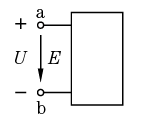
\includegraphics[width=1\textwidth]{p1-1-a.png}
    \caption*{(a)}
  \end{minipage}
  \begin{minipage}[t]{0.146\textwidth}
    \centering
    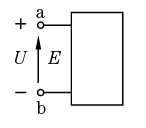
\includegraphics[width=1\textwidth]{p1-1-b.png}
    \caption*{(b)}
  \end{minipage}
  \begin{minipage}[t]{0.146\textwidth}
    \centering
    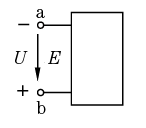
\includegraphics[width=1\textwidth]{p1-1-c.png}
    \caption*{(c)}
  \end{minipage}
  \begin{minipage}[t]{0.146\textwidth}
    \centering
    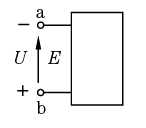
\includegraphics[width=1\textwidth]{p1-1-d.png}
    \caption*{(d)}
  \end{minipage}
  \caption*{题图 1-1}
\end{figure}

\paragraph{答} (a) $U=5{\rm V}, E=-5{\rm V}$;  \\

(b) $U=5{\rm V}, E=5{\rm V}$;  \\

(c) $U=-5{\rm V}, E=-5{\rm V}$;  \\

(d) $U=-5{\rm V}, E=5{\rm V}$.  \\

\paragraph{1-2}
\label{1-2}
分别求题图1-2(a)、(b)、(c)所示电路中的电压$U$和电流$I$。

\begin{figure}[!htb]
  \centering
  \begin{minipage}[t]{0.188\textwidth}
    \centering
    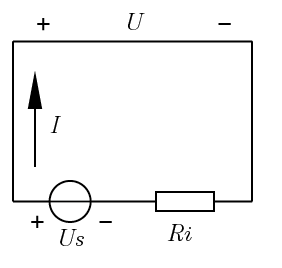
\includegraphics[width=1\textwidth]{p1-2-a.png}
    \caption*{(a) 短路}
  \end{minipage}
  \begin{minipage}[t]{0.192\textwidth}
    \centering
    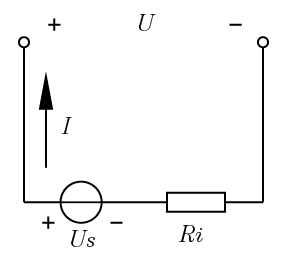
\includegraphics[width=1\textwidth]{p1-2-b.png}
    \caption*{(b) 开路}
  \end{minipage}
  \begin{minipage}[t]{0.180\textwidth}
    \centering
    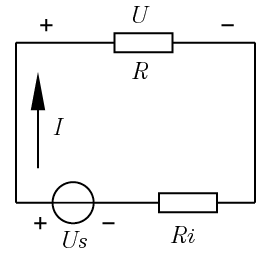
\includegraphics[width=1\textwidth]{p1-2-c.png}
    \caption*{(c) 接负载$R$}
  \end{minipage}
  \caption*{题图 1-2}
\end{figure}

\paragraph{解} (a) $I=\frac{U_s}{R_i}, U=0;$ \\

(b) $I=0, U=U_s; $ \\

(c) $I=\frac{U_s}{R+R_i}, U=IR=\frac{U_sR}{R+R_i}$ \\

\paragraph{1-9} \label{1-9}
分别求题图1-9(a)所示电路中的电压$U_{ab}$,图(b)电路中的电阻$R$,图(c)所示电路中的电压$U_s$和图(d)所示电路中的电流$I$。\\

\begin{figure}[!htb]
  \centering
  \begin{minipage}[t]{0.256\textwidth}
    \centering
    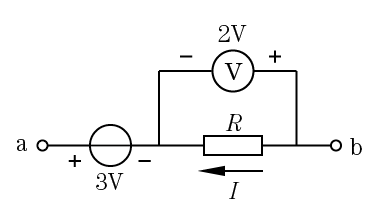
\includegraphics[width=1\textwidth]{p1-9-a.png}
    \caption*{(a)}
  \end{minipage}
  \begin{minipage}[t]{0.257\textwidth}
    \centering
    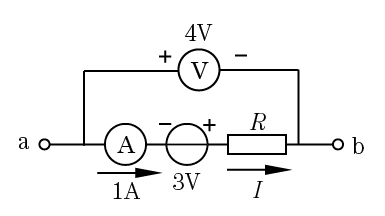
\includegraphics[width=1\textwidth]{p1-9-b.png}
    \caption*{(b)}
  \end{minipage} \\
  \centering
  \begin{minipage}[t]{0.254\textwidth}
    \centering
    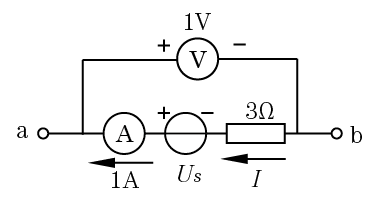
\includegraphics[width=1\textwidth]{p1-9-c.png}
    \caption*{(c)}
  \end{minipage}
  \begin{minipage}[t]{0.263\textwidth}
    \centering
    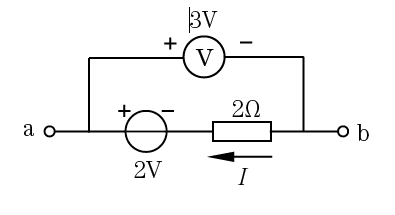
\includegraphics[width=1\textwidth]{p1-9-d.png}
    \caption*{(d)}
  \end{minipage}
  \caption*{题图 1-9}
\end{figure}

\paragraph{解}
(a) $U_{ab}=3-2=1{\rm V}; $ \\

(b) $R=\frac{4+3}{1}=7\Omega; $ \\

(c) $U_s=1+3=4{\rm V}; $ \\

(d) $I=\frac{2-3}{2}=-0.5{\rm A}. $ \\

\paragraph{1-10} \label{1-10}
求题图1-10所示电路中的电压$U_{\rm ab}$。 \\

\begin{figure}[!htb]
  \centering
  \begin{minipage}[t]{0.261\textwidth}
    \centering
    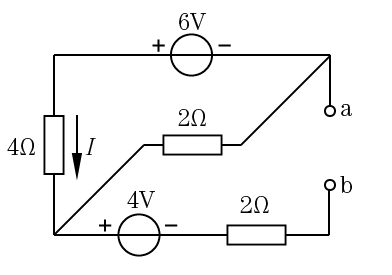
\includegraphics[width=1\textwidth]{p1-10-a.png}
    \caption*{(a)}
  \end{minipage}
  \begin{minipage}[t]{0.264\textwidth}
    \centering
    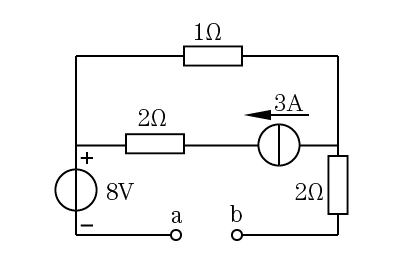
\includegraphics[width=1\textwidth]{p1-10-b.png}
    \caption*{(b)}
  \end{minipage}
  \caption*{题图 1-10}
\end{figure}

\paragraph{解}
\subparagraph{(a)}
设流过$4\Omega$电阻的电流为$I$, 则
$$I=\frac{6}{6}=1{\rm A} $$
$$U_{\rm ab}=-6+4+4=2{\rm V}$$
\subparagraph{(b)}
$U_{\rm ab}=-8+3\times 1=-5{\rm V}$

\paragraph{1-11}\label{1-11}
求题图1-11所示电路中的电压$U_{\rm AB}, U_{\rm BC}, U_{\rm CA}$和$U_{\rm BD}$。
\begin{figure}[!htb]
  \centering
  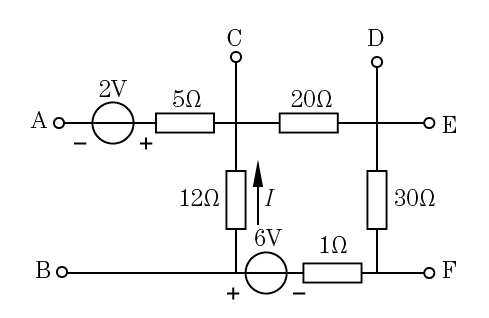
\includegraphics[width=0.326\textwidth]{p1-11.png}
  \caption*{题图 1-11}
\end{figure}

\paragraph{解}
$$ I = \frac{6}{63}=0.095{\rm A} $$
$$ U_{\rm AB}=-2-12I=-3.143{\rm V} $$
$$ U_{\rm BC}=12I=1.143{\rm V} $$
$$ U_{\rm CA}=2{\rm V} $$
$$ U_{\rm BD}=32I=3.048{\rm V} $$

\paragraph{1-12}\label{1-12}
题图1-12所示电路中,已知支路电压$U_1=10{\rm V}, U_2=5{\rm V}, U_4=-3{\rm V}, U_6=2{\rm V}, U_7=-3{\rm V}, U_{12}=8{\rm V}$。试确定其他可能求的电压。

\begin{figure}[!htb]
  \centering
  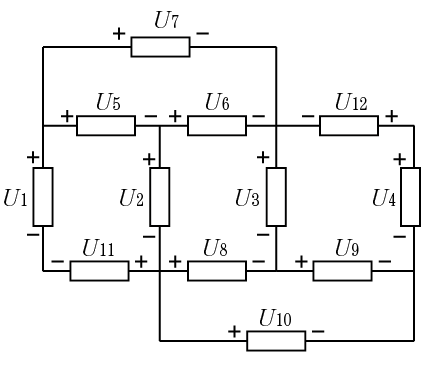
\includegraphics[width=0.291\textwidth]{p1-12.png}
  \caption*{题图 1-12}
\end{figure}

\paragraph{解}
$$ U_5=U_7-U_6=-5{\rm V} $$
$$ U_{11}=-U_2-U_5+U_1=10{\rm V} $$
$$ U_{10}=-U_2+U_6-U_{12}+U_4=-14{\rm V} $$

\paragraph{1-13} \label{1-13}
在题图1-12所示电路中,若各支路电流与对应支路电压的参考方向一直,并已知支路电流$I_1=1{\rm A}$, $I_3=1{\rm A}$, $I_4=5{\rm A}$, $I_7=-5{\rm A}$, $I_{10}=-3{\rm A}$。试确定其他可能求得的电流。

\begin{figure}[!htb]
  \centering
  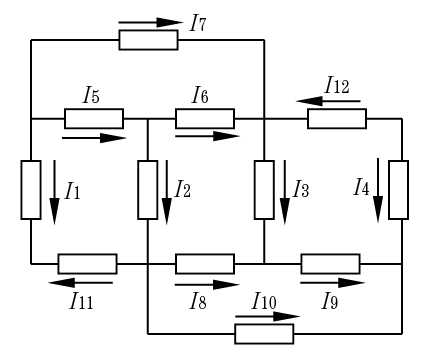
\includegraphics[width=0.292\textwidth]{p1-13.png}
  \caption*{图 1-13}
\end{figure}

\paragraph{解}
如图1-13所示,
$$ I_{12}=-I_4=-5{\rm A}$$
$$ I_9=-I_4-I_{10}=-2{\rm A}$$
$$ I_5=-I_1-I_7=4{\rm A}$$
$$ I_6=-I_7+I_3-I_{12}=11{\rm A}$$
$$ I_2=I_5-I_6=-7{\rm A}$$
$$ I_{11}=-I_1=-1{\rm A}$$
$$ I_8=I_2-I_{10}-I_{11}=-3{\rm A}$$

\paragraph{1-20} \label{1-20}
求题图1-20(a), (b)所示电路中所标出的各电压和电流。

\begin{figure}[!htb]
  \centering
  \begin{minipage}[t]{0.359\textwidth}
    \centering
    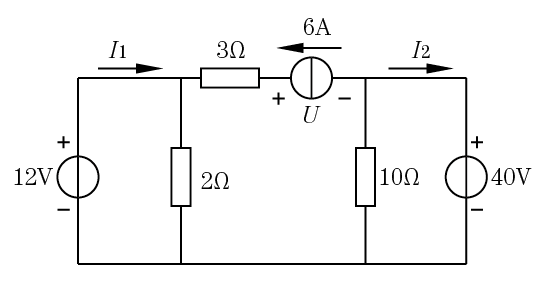
\includegraphics[width=1\textwidth]{p1-20-a.png}
    \caption*{(a)}
  \end{minipage}
  \begin{minipage}[t]{0.317\textwidth}
    \centering
    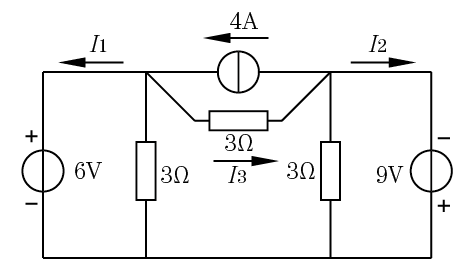
\includegraphics[width=1\textwidth]{p1-20-b.png}
    \caption*{(b)}
  \end{minipage}
  \caption*{题图 1-20}
\end{figure}

\paragraph{解}
\subparagraph{(a)}
$$ I_{2\Omega}=6{\rm A}$$
$$ I_1=6-6=0 $$
$$ I_{10\Omega}=4{\rm A}$$
$$ I_2=-6-=-10{\rm A}$$
$$ U=3 \times 6 + 12 - 40 = -10 {\rm V} $$
\subparagraph{(b)}
$$ I_3=\frac{6+9}{3}=5{\rm A} $$
$$ I_1=-\frac{6}{3} - 5 + 4 = -3 {\rm A} $$
$$ I_2=\frac{9}{3}+5-4=4{\rm A} $$

\paragraph{1-21} \label{1-21}
已知题图1-21所示电路中,电压$U=6{\rm V}$。求由电源端看进去的电阻$R_{\rm eq}$和电阻$R_1$的值。

\begin{figure}[!htb]
  \centering
  \begin{minipage}[t]{0.305\textwidth}
    \centering
    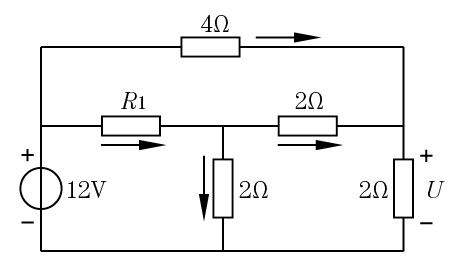
\includegraphics[width=1\textwidth]{p1-21.png}
    \caption*{题图 1-21}
  \end{minipage}
  \begin{minipage}[t]{0.296\textwidth}
    \centering
    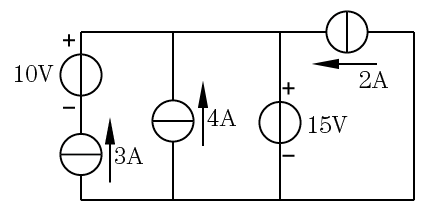
\includegraphics[width=1\textwidth]{p1-22.png}
    \caption*{题图 1-22}
  \end{minipage}
\end{figure}

\paragraph{解}
$$I_1=\frac{12-6}{4}=1.5{\rm A}$$
$$I_2=\frac{6}{2}-I_1=1.5{\rm A}$$
$$I_3=\frac{9}{2}=4.5{\rm A}$$
$$I_4=I_2+I_3=6{\rm A}$$
$$R_1=\frac{3}{6}=0.5\Omega$$
电源流出电流$$I_{\rm s}=I_1+I_4=7.5{\rm A}$$
等效电阻$$R_{\rm eq}=\frac{12}{2.5}=1.6\Omega$$

\paragraph{1-22}\label{1-22}
求题图1-22所示电路中各电源发出的功率。
\paragraph{解}
$$ I_{10 \rm V}=-3{\rm A}, P_{10 \rm V}=30{\rm W} $$
$$ U_{3 \rm A}=-5{\rm V}, P_{3 \rm A}=15{\rm W} $$
$$ I_{15 \rm V}=3+4+2=9{\rm A}, P_{15 \rm V}=-135{\rm W} $$
$$ U_{4 \rm A}=-15{\rm V}, P_{4 \rm A}=60{\rm W} $$
$$ U_{2 \rm A}=-15{\rm V}, P_{2 \rm A}=30{\rm W} $$

\paragraph{1-23}\label{1-23}
求题图1-23所示电路中负载吸收的功率。

\begin{figure}[!htb]
  \centering
  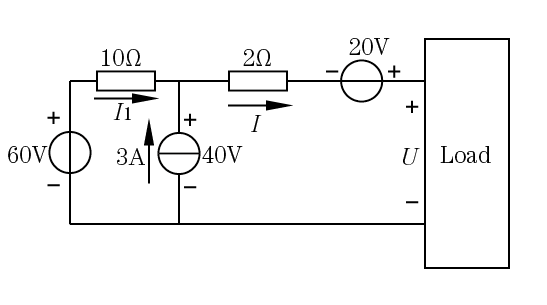
\includegraphics[width=0.365\textwidth]{p1-23.png}
  \caption*{图 1-23}
\end{figure}

\paragraph{解}
$$I_1=\frac{60-40}{10}=2{\rm A} $$
$$I=3+2=5{\rm A}$$
$$U=20-2\times 5+40=50{\rm V}$$
$$P=UI=250{\rm W} $$

\paragraph{1-27}\label{1-27}
求题图1-27所示电路中从电压源两端看进去的等效电阻$R_{\rm eq}$。

\begin{figure}[!htb]
  \centering
  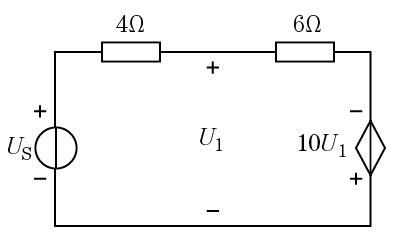
\includegraphics[width=0.271\textwidth]{p1-27.png}
  \caption*{图 1-27}
\end{figure}

\paragraph{解}
$$
    \begin{cases}
    U_{\rm s} = (4+6)I-10U_1 \\
    U_1 = 6I - 10U_1
    \end{cases}
$$
$$
    \therefore U_1=\frac{6}{11}I,
    U_{\rm s}=10I-\frac{60}{11}I = \frac{50}{11}I
$$
$$
    R_{\rm eq}=\frac{U_s}{I}=\frac{50}{11}\Omega=4.55\Omega
$$

\paragraph{1-33}\label{1-33}
已知题图1-33所示电路中,$R_1=40\Omega$, $R_{\rm e}=27\Omega$, $R_{\rm b}=150\Omega$, $\alpha=0.98$。求电压增益$u_2/u_1$和功率增益$p_2/p_1$。其中$p_1$是$u_1$输出的功率,$p_2$是$R_{\rm L}$吸收的功率。

\begin{figure}[!htb]
  \centering
  \begin{minipage}[t]{0.328\textwidth}
    \centering
    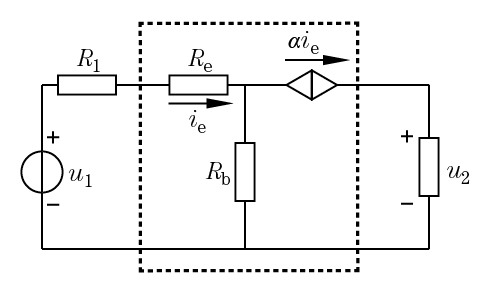
\includegraphics[width=1\textwidth]{p1-33.png}
    \caption*{题图 1-33}
  \end{minipage}
  \begin{minipage}[t]{0.379\textwidth}
    \centering
    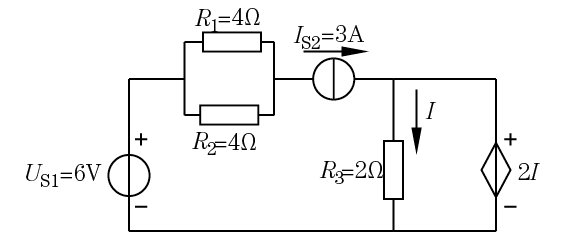
\includegraphics[width=1\textwidth]{p1-34.png}
    \caption*{题图 1-34}
  \end{minipage}
\end{figure}

\paragraph{解}
\begin{gather*}
    \begin{cases}
    U_1=(R_1+R_{\rm e})i_{\rm e}+R_{\rm b}(i_{\rm e}-\alpha i_{\rm e}) \\
    U_2=\alpha i_{\rm e}R_{\rm e}
    \end{cases} \\
    \therefore i_{\rm e}=\frac{U_1}{R_1+R_{\rm e}+R_{\rm b}(1-\alpha)}=\frac{U_1}{70} \\
    \therefore U_2=0.98 \times \frac{U_1}{70} \times 1500=21U_1 \\
    \therefore \frac{U_2}{U_1}=21 \\
    \frac{p_2}{p_1}=\frac{U_2 \cdot \alpha I_{\rm e}}{-U_1i_{\rm e}} = 21 \times 0.98 = 20.58
\end{gather*}

\paragraph{1-34}\label{1-34}
求题图1-34所示电路中各元件的功率,并校验功率守恒。

\paragraph{解}
\begin{gather*}
    I_{R_1}=1{\rm A}, I_{R_2}=2{\rm A} \\
    p_{R_1}=2{\rm W}, p_{R_2}=4{\rm W} \\
    p_{S_1}=-U_{S_1} \cdot I_{S_2}=-18 {\rm W} \\
    \text{由} I+2I=3{\rm A}\text{知}, I=1{\rm A}, U_{R_3}=2{\rm V} \\
    p_{R_3}=2{\rm W} \\
    U_{S_2}=U_{S_1}-2-2=2{\rm V} \\
    p_{S_2}=2 \times 3 = 6{\rm W} \\
    p_{\rm CS}=4{\rm W} \\
    \therefore p_{\rm CS}+p_{R_1}+p_{R_2}+p_{R_3}+ p_{S_1}+p_{S_2}=0
\end{gather*}

\paragraph{2-1}\label{2-1}
求题图2-1所示各电路的入端电阻$R_{\rm AB}$。

\begin{figure}[!htb]
  \centering
  \begin{minipage}[t]{0.192\textwidth}
    \centering
    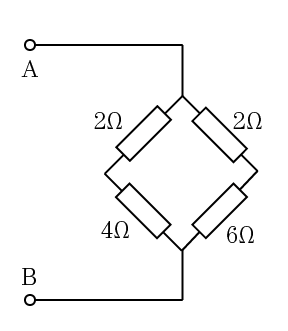
\includegraphics[width=1\textwidth]{p2-1-a.png}
    \caption*{(a)}
  \end{minipage}
  \begin{minipage}[t]{0.184\textwidth}
    \centering
    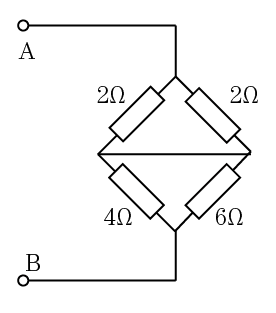
\includegraphics[width=1\textwidth]{p2-1-b.png}
    \caption*{(b)}
  \end{minipage}
  \begin{minipage}[t]{0.208\textwidth}
    \centering
    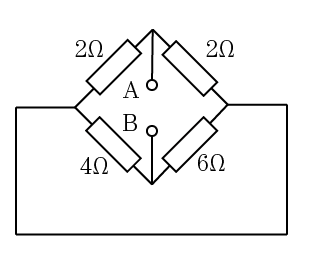
\includegraphics[width=1\textwidth]{p2-1-c.png}
    \caption*{(c)}
  \end{minipage} \\
  \centering
  \begin{minipage}[t]{0.195\textwidth}
    \centering
    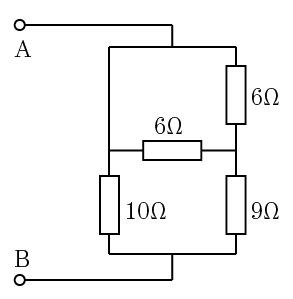
\includegraphics[width=1\textwidth]{p2-1-d.png}
    \caption*{(d)}
  \end{minipage}
  \begin{minipage}[t]{0.177\textwidth}
    \centering
    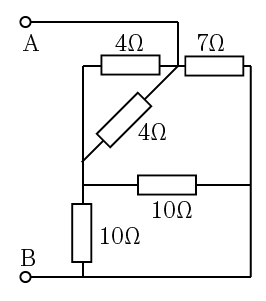
\includegraphics[width=1\textwidth]{p2-1-e.png}
    \caption*{(e)}
  \end{minipage}
  \begin{minipage}[t]{0.219\textwidth}
    \centering
    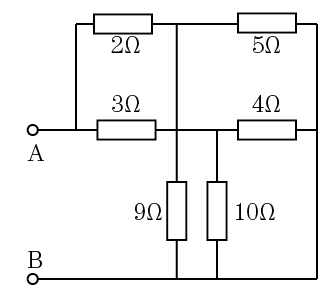
\includegraphics[width=1\textwidth]{p2-1-f.png}
    \caption*{(f)}
  \end{minipage}
  \caption*{题图 2-1}
\end{figure}

\paragraph{解}
\subparagraph{(a)}
$R = (2+4)//(2+6)=\frac{7}{24}\Omega=3.43\Omega$
\subparagraph{(b)}
$R=2//2+4//6=\frac{17}{5}\Omega=3.4\Omega$
\subparagraph{(c)}
$R=2//2+4//6=\frac{17}{5}\Omega=3.4\Omega$
\subparagraph{(d)}
$R=(6//6+9)//10=\frac{60}{11}\Omega=5.45\Omega$
\subparagraph{(e)}
$R=(4//4+10//10)//7=3.5\Omega$
\subparagraph{(f)}
$R=(2+5//9)/(3+4//10)=\frac{73}{14}//\frac{41}{7}=2.76\Omega$

\paragraph{2-3} \label{2-3}
求题图2-3所示各电路的入端电阻$R_{ab}$。

\begin{figure}[!htb]
  \centering
  \begin{minipage}[t]{0.243\textwidth}
    \centering
    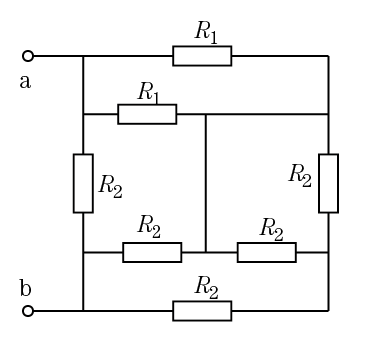
\includegraphics[width=1\textwidth]{p2-3-a.png}
    \caption*{(a)}
  \end{minipage}
  \begin{minipage}[t]{0.217\textwidth}
    \centering
    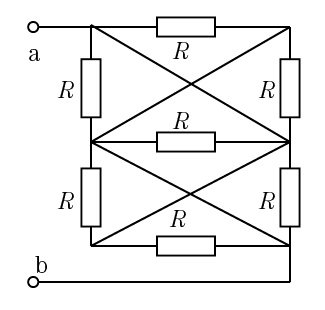
\includegraphics[width=1\textwidth]{p2-3-b.png}
    \caption*{(b)}
  \end{minipage}
  \begin{minipage}[t]{0.270\textwidth}
    \centering
    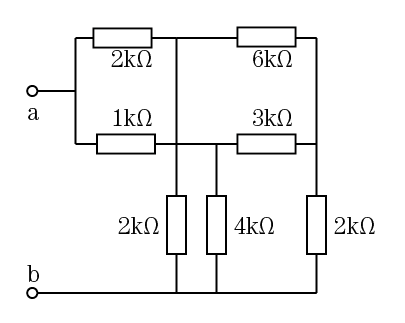
\includegraphics[width=1\textwidth]{p2-3-c.png}
    \caption*{(c)}
  \end{minipage}
  \caption*{题图 2-3}
\end{figure}

\paragraph{解}
\subparagraph{(a)} 对下方三个$R_2$进行Y-$\Delta$变换。如图2-3-a所示。
\begin{figure}[!htb]
  \centering
  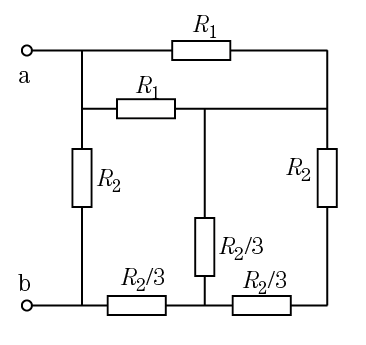
\includegraphics[width=0.244\textwidth]{p2-3-a-sol.png}
  \caption*{图 2-3-a}
\end{figure} \\
则
\begin{align*}
R_{\rm ab} &=
R_2//[(R_1//R_1)+
\frac{R_2}{3}//(R_2+\frac{R_2}{3})+\frac{R_2}{3}] \\
&= R_2//(\frac{1}{2}R_1+\frac{3}{5}R_2) \\
&= \frac{R_2(5R_1+6R_2)}{5R_1+16R_2}
\end{align*}
\subparagraph{(b)} 该电路图等同于七个$R$并联。
$R_{\rm ab}=R//R//R//R//R//R//R=\frac{1}{7}R$
\subparagraph{(c)} 由于图中两个Y形电路中电阻成比例,因而可以将对应电阻视为并联。如图2-3-c所示。
\begin{figure}[!htb]
  \centering
  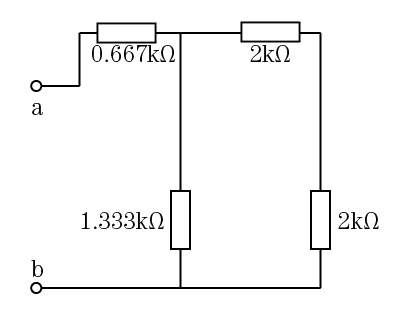
\includegraphics[width=0.267\textwidth]{p2-3-c-sol.png}
  \caption*{图 2-3-c}
\end{figure} \\
则
$R_{\rm ab}=(4//\frac{4}{3})+\frac{2}{3}=1.67\Omega$

\paragraph{2-4}\label{2-4}
求题图2-4所示各电路的入端电阻$R_{AB}$。图中各电阻值均为$1\Omega$。

\begin{figure}[!htb]
  \centering
  \begin{minipage}[t]{0.251\textwidth}
    \centering
    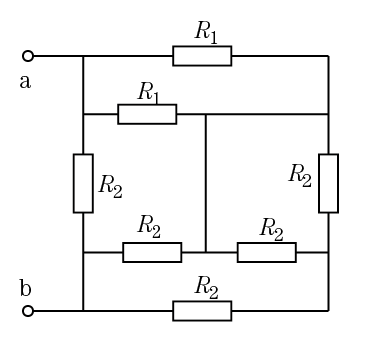
\includegraphics[width=1\textwidth]{p2-3-a.png}
    \caption*{(a)}
  \end{minipage}
  \begin{minipage}[t]{0.212\textwidth}
    \centering
    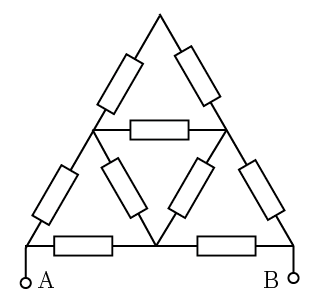
\includegraphics[width=1\textwidth]{p2-4-b.png}
    \caption*{(b)}
  \end{minipage}
  \begin{minipage}[t]{0.193\textwidth}
    \centering
    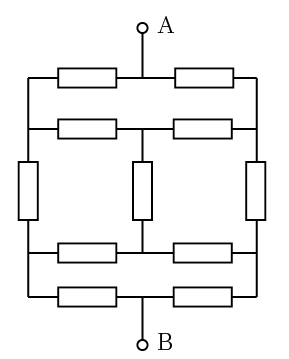
\includegraphics[width=1\textwidth]{p2-4-c.png}
    \caption*{(c)}
  \end{minipage}
  \caption*{题图 2-4}
\end{figure}

\subparagraph{(a)}
由电桥平衡,知
$R_{\rm AB}=2//2//1=0.5\Omega$
\subparagraph{(b)}
首先将上部的$2R$和$R$并联得到$\frac{2}{3}R$电阻,然后将左下部分和右下部分的$\Delta$形电路分别做Y-$\Delta$变换。如图2-4-b所示。则有
\begin{figure}[!htb]
  \centering
  \begin{minipage}[t]{0.255\textwidth}
    \centering
    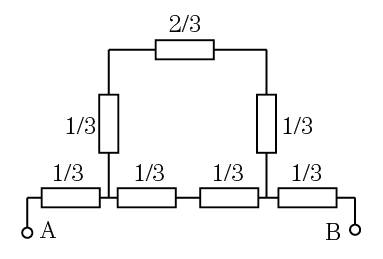
\includegraphics[width=1\textwidth]{p2-4-b-sol.png}
    \caption*{图 2-4-b}
  \end{minipage}
  \begin{minipage}[t]{0.173\textwidth}
    \centering
    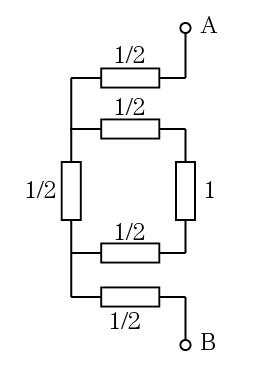
\includegraphics[width=1\textwidth]{p2-4-c-sol.png}
    \caption*{图 2-4-c}
  \end{minipage}
\end{figure}
$$R_{\rm AB}=
\frac{1}{3}+\frac{4}{3}//\frac{2}{3}+\frac{1}{3}=1.11\Omega$$
\subparagraph{(c)}
由对称性,可以将该电路左右对折,重合者视为并联。如图2-3-c所示。则
$$R_{\rm AB}=0.5+0.5//2+0.5=1.4\Omega$$

\paragraph{2-6} \label{2-6}
试将题图2-6中各电路化成最简单形式。

\begin{figure}[!htb]
  \centering
  \begin{minipage}[t]{0.212\textwidth}
    \centering
    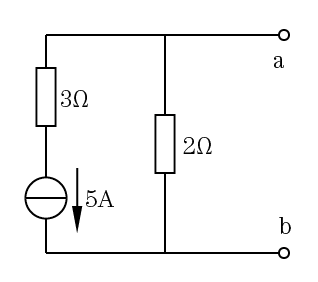
\includegraphics[width=1\textwidth]{p2-6-a.png}
    \caption*{(a)}
  \end{minipage}
  \begin{minipage}[t]{0.195\textwidth}
    \centering
    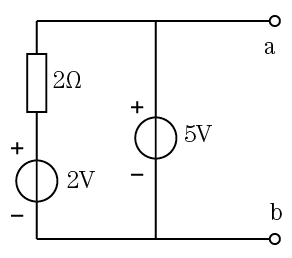
\includegraphics[width=1\textwidth]{p2-6-b.png}
    \caption*{(b)}
  \end{minipage} \\
  \centering
  \begin{minipage}[t]{0.221\textwidth}
    \centering
    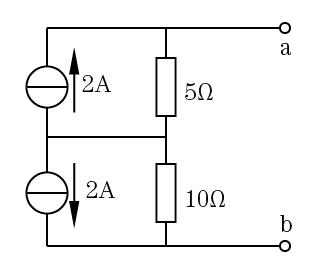
\includegraphics[width=1\textwidth]{p2-6-c.png}
    \caption*{(c)}
  \end{minipage}
  \begin{minipage}[t]{0.253\textwidth}
    \centering
    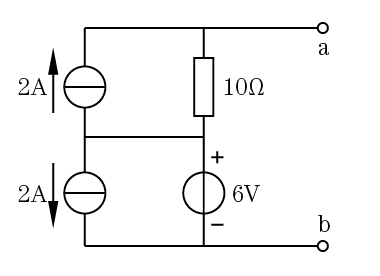
\includegraphics[width=1\textwidth]{p2-6-d.png}
    \caption*{(d)}
  \end{minipage}
  \caption*{题图 2-6}
\end{figure}
\paragraph{解}设从a端流入电流为$I$, $U=U_{ab}$。
\subparagraph{(a)}
$U=(I-5)\cdot 2=2I-10$,如图2-6-a所示。
\subparagraph{(b)}
$U=5{\rm V}$,如图2-6-b所示。
\subparagraph{(c)}
$U=5(I+2)+10(I-2)=15I-10$,如图2-6-c所示。
\subparagraph{(d)}
$U=6+(2+I)\cdot 10=26+10I$,如图2-6-d所示。
\begin{figure}[!htb]
  \centering
  \begin{minipage}[t]{0.179\textwidth}
    \centering
    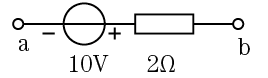
\includegraphics[width=1\textwidth]{p2-6-a-sol.png}
    \caption*{图 2-6-a}
  \end{minipage}
  \begin{minipage}[t]{0.177\textwidth}
    \centering
    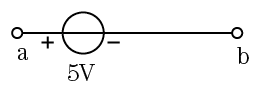
\includegraphics[width=1\textwidth]{p2-6-b-sol.png}
    \caption*{图 2-6-b}
  \end{minipage} \\
  \centering
  \begin{minipage}[t]{0.165\textwidth}
    \centering
    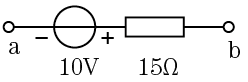
\includegraphics[width=1\textwidth]{p2-6-c-sol.png}
    \caption*{图 2-6-c}
  \end{minipage}
  \begin{minipage}[t]{0.172\textwidth}
    \centering
    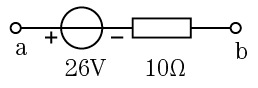
\includegraphics[width=1\textwidth]{p2-6-d-sol.png}
    \caption*{图 2-6-d}
  \end{minipage}
\end{figure}

\paragraph{2-12}\label{2-12}
题图2-12所示电路中,已知电压源电压$U_{\rm S1}=U_{\rm S6}=20{\rm V}$, $U_{\rm S2}=U_{\rm S5}=10{\rm V}$, $U_{\rm S4}=15{\rm V}$,电流源电流$I_{\rm S3}=10{\rm A}$,电阻$R_1=10\Omega$, $R_2=5\Omega$, $R_3=1\Omega$, $R_4=2\Omega$, $R_5=R_6=4\Omega$。试求电路中各支路的电流。

\begin{figure}[!htb]
    \centering
    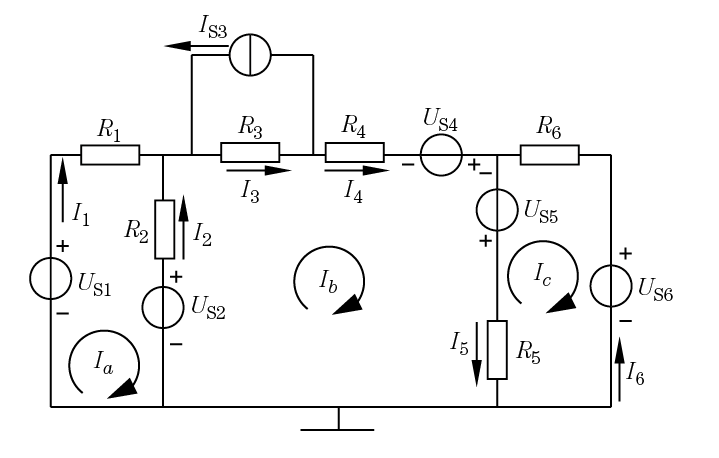
\includegraphics[width=0.479\textwidth]{p2-12.png}
    \caption*{题图 2-12}
\end{figure}

\paragraph{解}如图所示,设三个回路电流分别为$I_a, I_b, I_c$。
\begin{gather*}
    \left\{ \begin{aligned}
    -U_{\rm S1}+R_1I_a+R_2(I_a-I_b)+U_{\rm S2} &= 0 \\
    -U_{\rm S2}+R_2(I_b-I_a)+(I_b+I_{\rm S3})R_3+R_4I_b -U_{\rm S4}-U_{\rm S5}+(I_b-I_c)R_5 & = 0 \\
    U_{\rm S5}+R_6I_c+U_{\rm S6}+(I_c-I_b)R_5 & = 0
    \end{aligned}
    \right. \\
    \therefore I_a=1.2{\rm A}, I_b=1.6{\rm A}, I_c=-2.95{\rm A} \\
    \therefore I_1=1.2{\rm A}, I_2=0.4{\rm A}, I_3=11.6{\rm A}, I_4=1.6{\rm A}, I_5=4.55{\rm A}, I_6=2.95{\rm A}
\end{gather*}

\paragraph{2-20} \label{2-20}
用电阻的Y-$\Delta$变换方法,求题图2-20所示电路的入端电阻$R_{\rm AB}$。

\begin{figure}[!htb]
  \centering
  \begin{minipage}[t]{0.269\textwidth}
    \centering
    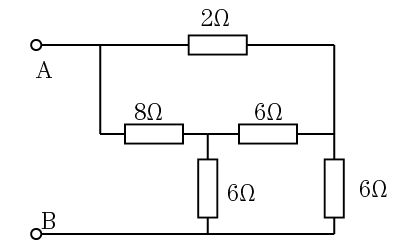
\includegraphics[width=1\textwidth]{p2-20-a.png}
    \caption*{(a)}
  \end{minipage}
  \begin{minipage}[t]{0.256\textwidth}
    \centering
    \includegraphics[width=1\textwidth]{p2-20-b.png}
    \caption*{(b)}
  \end{minipage} \\
  \centering
  \begin{minipage}[t]{0.203\textwidth}
    \centering
    \includegraphics[width=1\textwidth]{p2-20-c.png}
    \caption*{(c)}
  \end{minipage}
  \begin{minipage}[t]{0.334\textwidth}
    \centering
    \includegraphics[width=1\textwidth]{p2-20-d.png}
    \caption*{(d)}
  \end{minipage}
  \caption*{题图 2-20}
\end{figure}

\paragraph{解}
\subparagraph{(a)}对三个$6\Omega$做Y-$\Delta$变换。如图2-20-a所示。则$R_{\rm AB}=2+10//4=4.86\Omega$
\begin{figure}[!htb]
  \centering
  \begin{minipage}[t]{0.241\textwidth}
    \centering
    \includegraphics[width=1\textwidth]{p2-20-a-sol.png}
    \caption*{图 2-20-a}
  \end{minipage}
  \begin{minipage}[t]{0.254\textwidth}
    \centering
    \includegraphics[width=1\textwidth]{p2-20-b-sol.png}
    \caption*{图 2-20-b}
  \end{minipage}
  \begin{minipage}[t]{0.187\textwidth}
    \centering
    \includegraphics[width=1\textwidth]{p2-20-c-sol.png}
    \caption*{图 2-20-c}
  \end{minipage}
\end{figure}

\subparagraph{(b)}对$6\Omega, 4\Omega, 10\Omega$做Y-$\Delta$变换。如图2-20-b所示。则
$$R_ {\rm AB}
=(5//31)//(2//12.4+2//20.667)
=4.306//(1.722+1.823)=1.944\Omega$$

\subparagraph{(c)}对$1\Omega, 4\Omega, 5\Omega$做Y-$\Delta$变换。如图2-20-c所示。则
$R_ {\rm AB}=1//1+2=2.5\Omega$

\subparagraph{(d)}先对$3\Omega, 4\Omega, 5\Omega$做Y-$\Delta$变换。如图2-20-d(1)所示。之后对$7\Omega, 1\Omega, 8.25\Omega$做Y-$\Delta$变换。如图2-20-d(2)所示。
$$\therefore R_{\rm AB}=8.431//10.174+3.554=8.164\Omega$$

\begin{figure}[!htb]
  \centering
  \begin{minipage}[t]{0.334\textwidth}
    \centering
    \includegraphics[width=1\textwidth]{p2-20-d-sol1.png}
    \caption*{图 2-20-d (1)}
  \end{minipage}
  \begin{minipage}[t]{0.334\textwidth}
    \centering
    \includegraphics[width=1\textwidth]{p2-20-d-sol2.png}
    \caption*{图 2-20-d (2)}
  \end{minipage}
\end{figure}

\end{document} 